\documentclass[11pt,t,usepdftitle=false,aspectratio=169]{beamer}
%% ------------------------------------------------------------------
%% - aspectratio=43: Set paper aspect ratio to 4:3.
%% - aspectratio=169: Set paper aspect ratio to 16:9.
%% ------------------------------------------------------------------

%% Add packages
\usepackage{eso-pic}


\usetheme[nototalframenumber,foot,logo]{uibk}
%% ------------------------------------------------------------------
%% - foot: Add a footer line for conference name and date.
%% - logo: Add the university logo in the footer (only if 'foot' set).
%% - bigfoot/sasquatch: Larger font size in footer.
%% - nototalslidenumber: Hide the total number of slides (only if 'foot' set)
%% - license: Add CC-BY license symbol to title slide (e.g., for conference uploads)
%%   (TODO: At the moment no other licenses are supported.)
%% - licenseall: Add CC-BY license symbol to all subsequent slides slides
%% - url: use \url{} rather than \href{} on the title page
%% ------------------------------------------------------------------

%% Set the size of the footer text
\setbeamerfont{footline}{size*={6pt}{6pt},parent=normal text}

%% ------------------------------------------------------------------
%% The official corporate colors of the university are predefined and
%% can be used for e.g., highlighting something. Simply use
%% \color{uibkorange} or \begin{color}{uibkorange} ... \end{color}
%% Defined colors are:
%% - uibkblue, uibkbluel, uibkorange, uibkorangel, uibkgray, uibkgraym, uibkgrayl
%% The frametitle color can be easily adjusted e.g., to black with
%% \setbeamercolor{titlelike}{fg=black}
%% ------------------------------------------------------------------

\setbeamercolor{verbcolor}{fg=uibkorange}

%% ------------------------------------------------------------------
%% Setting a highlight color for verbatim output such as from
%% the commands \pkg, \email, \file, \dataset 
%% ------------------------------------------------------------------


%% information for the title page ('short title' is the pdf-title that is shown in viewer's titlebar)
\title[HyPA]{HyPA: A Hybrid Proactive Autoscaler}
\subtitle{Area: Proactive Scaling of Containerized Orchestration Environments}

%('short author' is the pdf-metadata Author)
%% If multiple authors are required and the font size is too large you
%% can overrule the font size of author and url by calling:
%\setbeamerfont{author}{size*={10pt}{10pt},series=\mdseries}
%\setbeamerfont{url}{size*={10pt}{10pt},series=\mdseries}
\author[Dominik Gratz \& René Hueber]{Dominik Gratz, René Hueber\\[3mm]{\small Supervisors: Zahra Najafabadi Samani, PhD \\ \hspace{20mm} Juan Aznar Poveda, PhD}}


\footertext{Department of Computer Science \space - \space Bachelor Thesis \space - \space HyPA \space - \space October 3, 2023}

\headerimage{3}
%% ------------------------------------------------------------------
%% The theme offers four different header images based on the
%% corporate design of the university of innsbruck. Currently
%% 1, 2, 3 and 4 is allowed as input to \headerimage{...}. Default
%% or fallback is '1'.
%% ------------------------------------------------------------------


\begin{document}

%% ALTERNATIVE TITLEPAGE
%% The next block is how you add a titlepage with the 'nosectiontitlepage' option, which switches off
%% the default behavior of creating a titlepage every time a \section{} is defined.
%% Then you can use \section{} as it's originally intended, including a table of contents.
% \usebackgroundtemplate{\includegraphics[width=\paperwidth,height=\paperheight]{titlebackground.pdf}}
% \begin{frame}[plain]
%     \titlepage
% \end{frame}
% \addtocounter{framenumber}{-1}
% \usebackgroundtemplate{}}

%% Table of Contents, if wanted:
%% this requires the 'nosectiontitlepage' option and setting \section{}'s as you want them to appear here.
%% Subsections and subordinates are suppressed in the .sty at the moment, search
%% for \setbeamertemplate{subsection} and replace the empty {} with whatever you want.
%% Although it's probably too much for a presentation, maybe for a lecture.
% \begin{frame}
%     \vspace*{1cm plus 1fil}
%     \tableofcontents
%     \vspace*{0cm plus 1fil}
% \end{frame}


%% this sets the first PDF bookmark and triggers generation of the title page
\section{HyPA: A Hybrid Proactive Autoscaler}


%% this just generates PDF bookmarks
\subsection{The trend towards VoIP}
%% first slide
\begin{frame}
	\frametitle{The trend towards {\color{uibkorange} VoIP}}
	
	\begin{columns}
		\begin{column}{0.4\textwidth}	
			\begin{itemize}
				\item No more classic telephony
				\item No fixed wiring
				\item Migrate into the cloud
				\item Many supported protocols:
				\begin{itemize}
					\item SIP
					\item H.323
					\item RTP
					\item WebRTC
				\end{itemize}
				\item Challenges:
				\begin{itemize}
					\item Efficiency
					\item Scalability
					\item Maintenance
				\end{itemize}
			\end{itemize}
		\end{column}
		
		\begin{column}{0.6\textwidth}
			\begin{figure}
				\centering
				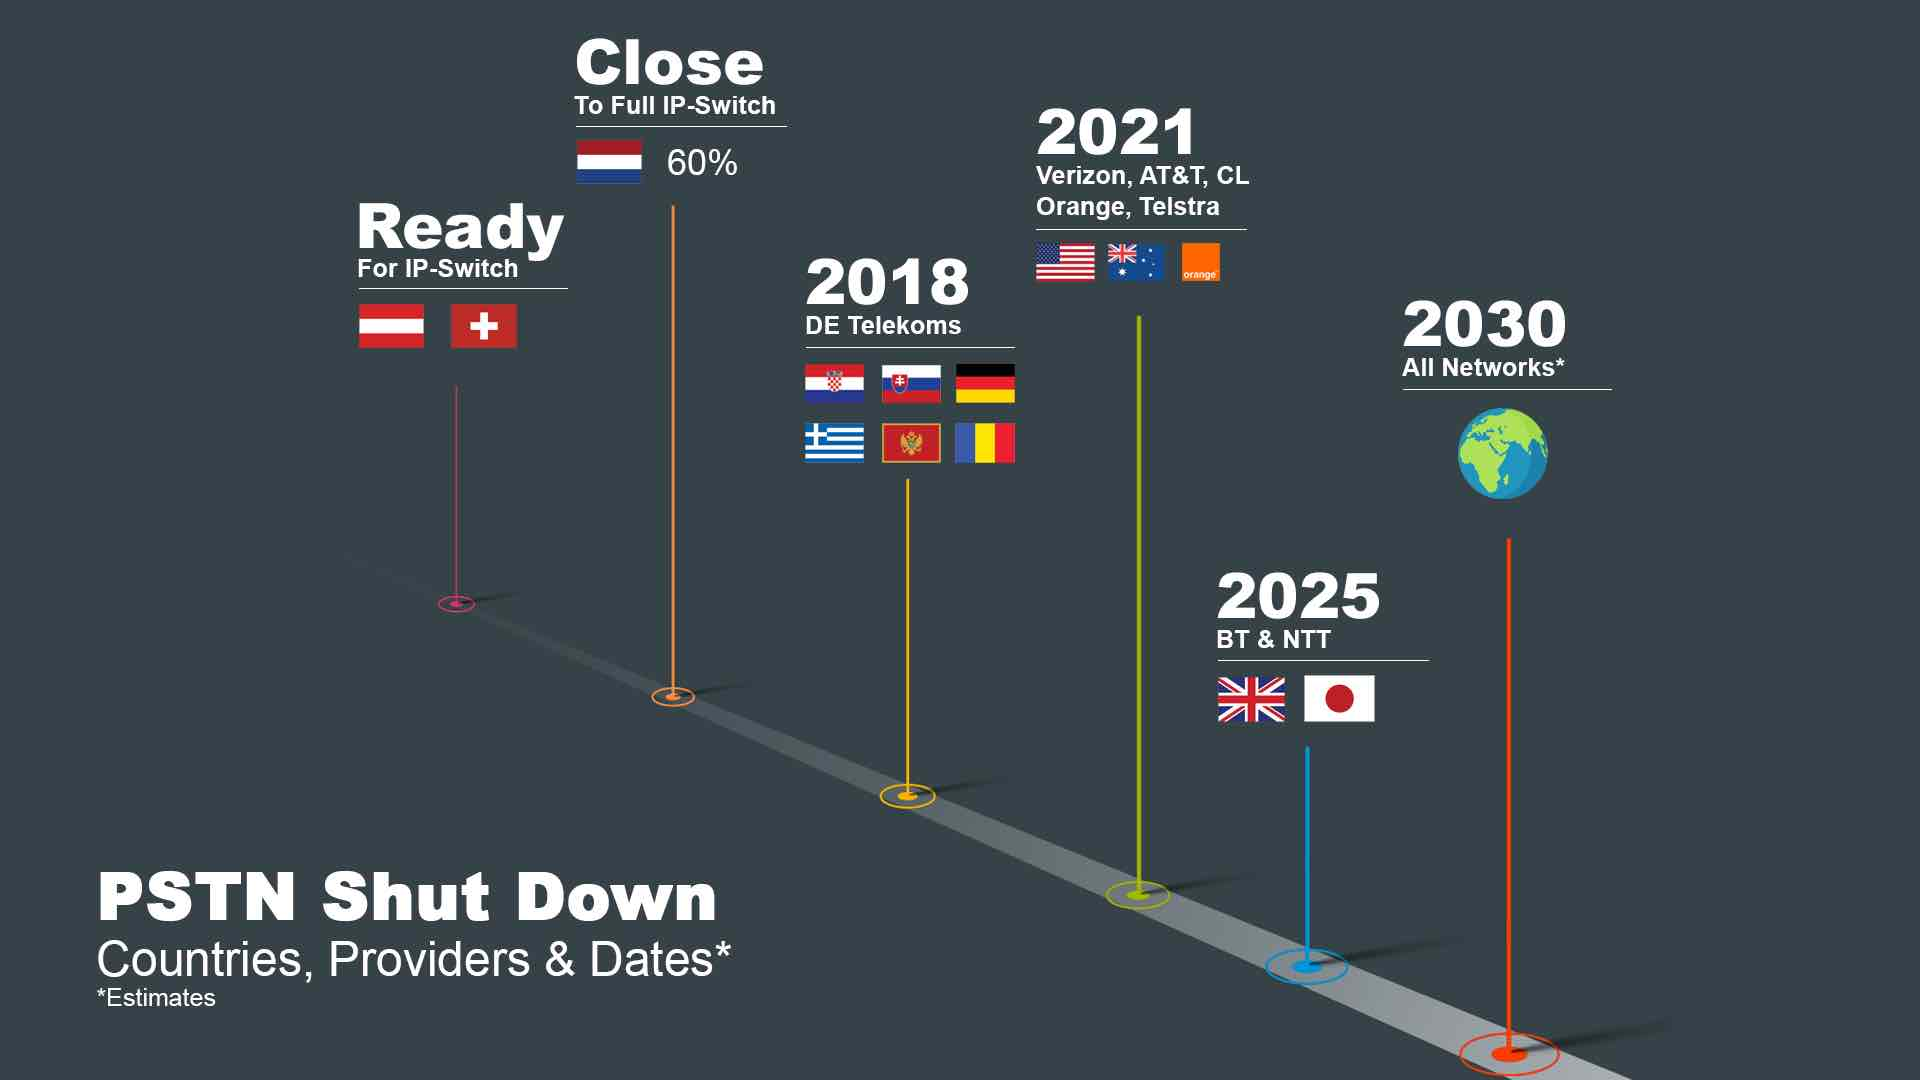
\includegraphics[width=1\textwidth]{_images/pstn_shutdown.jpg}
				\caption{PSTN Shut Down (As of 2016) \cite{bib_pstn_shutdown}}
			\end{figure}
		\end{column}
	\end{columns}
\end{frame}


\subsection{Cooperation with World-Direct}
\begin{frame}
	\frametitle{Cooperation with {\color{uibkblue} World-Direct}}
	
	\AddToShipoutPicture*{\put(325,200){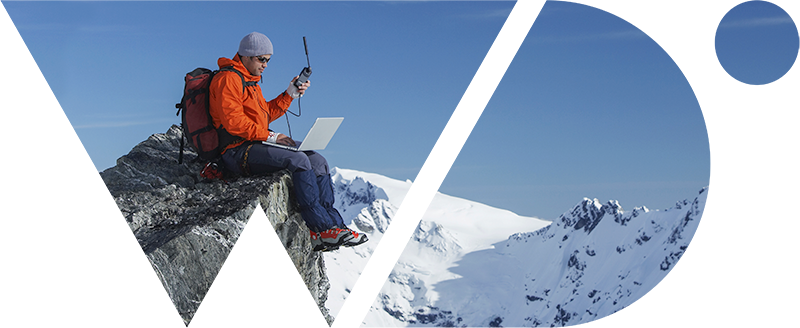
\includegraphics[width=4cm]{_images/world_direct_uc.png}}}
	
	\begin{itemize}
		\item Subsidiary company of A1
		\item Manages over 90.000 VoIP ports
		\item Transitions its telephone infrastructure to \textbf{\color{uibkorange} Kubernetes}
		\begin{itemize}
			\item Microservices
			\item API-first approach
			\item \textbf{{\color{uibkorange} Zero-Downtime}} architecture
		\end{itemize}
	\end{itemize}
	
	\begin{columns}
		\begin{column}{0.5\textwidth}		
			\begin{block}{Pros}
				\begin{itemize}
					\item Less complexity on the tenant side
					\item Central maintenance
					\item High flexibility and \textbf{\color{uibkorange} scalability}
				\end{itemize}
			\end{block}
		\end{column}
		
		\begin{column}{0.5\textwidth}		
			\begin{block}{Cons}
				\begin{itemize}
					\item Complex infrastructure
					\item Efficient architectures necessary
					\item \textbf{\color{red} Timely scaling}
				\end{itemize}
			\end{block}
		\end{column}
	\end{columns}
\end{frame}


\subsection{The specific problem: Scaling in real time}
\begin{frame}
	\frametitle{The specific problem: Scaling in {\color{uibkorange} real time}}
	
	\begin{itemize}
		\item High call traffic: 
		\begin{itemize}
			\item Increased load on the telephone system core
			\item Latency spikes
			\item Call cancellations
		\end{itemize}
	
		\item Scaling methods:
		\begin{itemize}
			\item Variable number of instances $\rightarrow$ \textbf{\color{uibkorange} horizontal}
			\item Variable CPU/memory assignment of a instance $\rightarrow$ \textbf{\color{uibkorange} vertical}
			\item Combining both approaches $\rightarrow$ \textbf{\color{uibkorange} hybrid}
		\end{itemize}
	
		\item \textbf{\color{uibkorange} Reactive} scaling is not enough:
		\begin{itemize}
			\item Static thresholds
			\item Scaling after the system is \textbf{\color{red} already compromised}
			\item Unusable for real-time applications
		\end{itemize}
	\end{itemize}
\end{frame}

\begin{frame}
	\frametitle{Example load test - Low traffic}
	
	\begin{figure}
		\centering
		\vspace*{-0.5cm}
		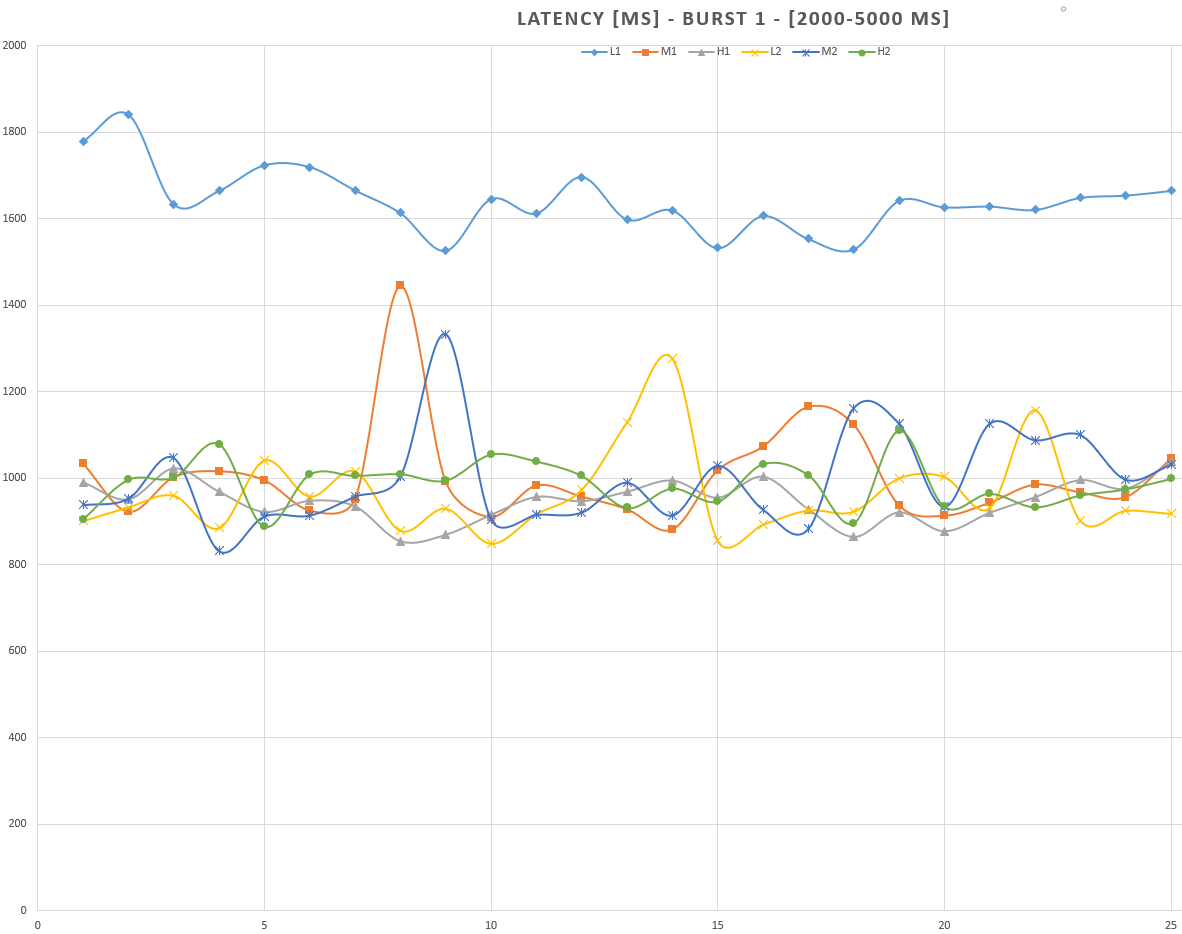
\includegraphics[width=13cm,height=7.2cm]{_images/load_low.png}
	\end{figure}
\end{frame}

\begin{frame}
	\frametitle{Example load test - High traffic}
	
	\begin{figure}
		\centering
		\vspace*{-0.5cm}
		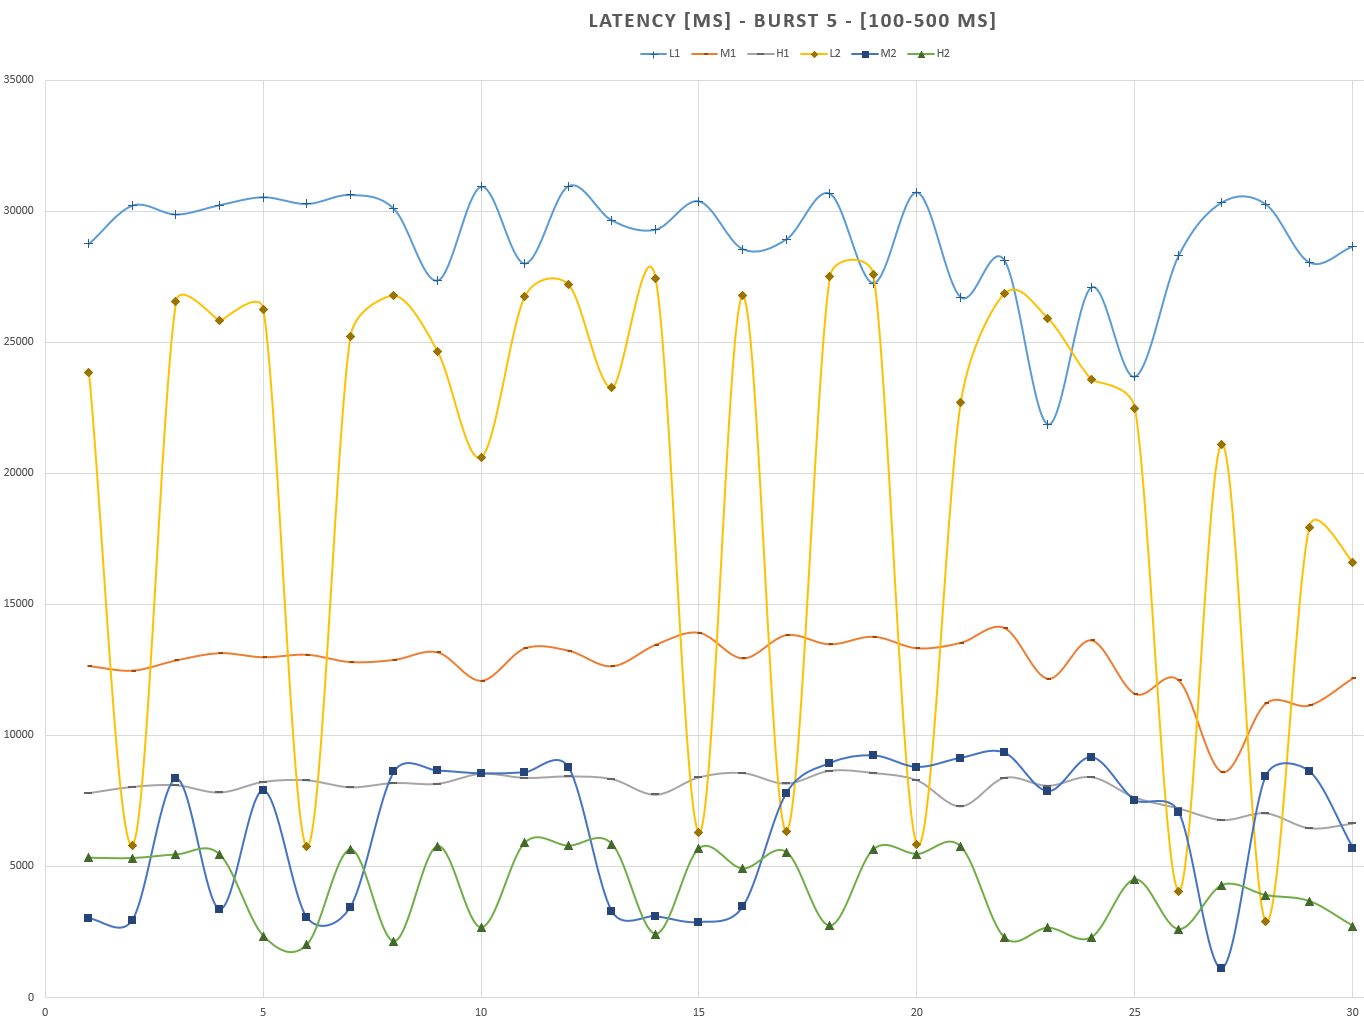
\includegraphics[width=13cm,height=7.2cm]{_images/load_high.png}
	\end{figure}
\end{frame}


\subsection{Proactive scaling}
\begin{frame}
	\frametitle{{\color{uibkorange} Proactive} scaling}
	
	\begin{itemize}
		\item Predict future resource needs $\rightarrow$ scale \textbf{\color{uibkorange} preemptively}
		\item Ensuring \textbf{\color{uibkorange} sufficient} resources during service lifetime
		\item Different models:
		\begin{itemize}
			\item Statistical $\rightarrow$ easy but \textbf{\color{red} slow} (ARMA, ARIMA, etc.)
			\item ML based models $\rightarrow$ complex but \textbf{\color{uibkorange} fast}
		\end{itemize}
	\end{itemize}
	
	\smallskip
	
	\begin{block}{Related work}
		\begin{itemize}
			\item Online Workload Burst Detection for Efficient Predictive Autoscaling of Applications \cite{bib_online_workload_burst_detection}
			
			\item Machine learning-based auto-scaling for containerized applications \cite{bib_ml_scaling_containerized_applications}
			
			\item Automatic Cloud Resource Scaling Algorithm based
			on Long Short-Term Memory Recurrent Neural Network \cite{bib_cloud_resource_scaling_lstm}
		\end{itemize}
	\end{block}
\end{frame}


\subsection{Thesis goal}
\begin{frame}
	\frametitle{Thesis goal}
	
	\begin{columns}
		\begin{column}{0.55\textwidth}
			\begin{block}{\textbf{HyPA}}
				\begin{itemize}
					\item \textbf{\color{uibkorange} Hy}brid scaling:
					\begin{itemize}
						\item Horizontal $\rightarrow$ number of instances
						\item Vertical $\rightarrow$ resource assignment
					\end{itemize}
					\item \textbf{\color{uibkorange} P}roactive approach:
					\begin{itemize}
						\item Reduce call latency
					\end{itemize}
					\item \textbf{\color{uibkorange} A}utoscaler:
					\begin{itemize}
						\item Automatically scale services at runtime
					\end{itemize}
				\end{itemize}
			\end{block}
		\end{column}
		
		\begin{column}{0.45\textwidth}
			\begin{block}{\textbf{Challenges}}
				\begin{itemize}
					\item Handling sporadic \textbf{\color{red} bursts}
					\item Resource \textbf{\color{red} conservation}
					\item Mitigating scaling \textbf{\color{red} oscillation}
					\item Ensuring no scaling \textbf{\color{red} downtime}
				\end{itemize}
			\end{block}
		\end{column}
	\end{columns}
\end{frame}


\subsection{Proposed method}
\begin{frame}
	\frametitle{Proposed method}
	
	\begin{alertblock}{Reinforcement Learning Model}
		\begin{itemize}
			\item Environment composed of:
			\begin{itemize}
				\item Burst detection $\rightarrow$ statistical
				\item Workload prediction $\rightarrow$ LSTM
				\item Data/Metric connectors
			\end{itemize}
			
			\item Environment designed for containerized orchestration environments
			\item Custom reward function
		\end{itemize}
	\end{alertblock}
	
	\begin{block}{Deployment}
		\begin{itemize}
			\item Train with synthetic data $\rightarrow$ automatic test pipeline
			\item Deploy in tenant namespace
			\item Models learns call \textbf{\color{uibkorange} patterns} of the tenant
		\end{itemize}
	\end{block}
\end{frame}


\subsection{Milestones}
\begin{frame}
	\frametitle{Milestones}
	
	\begin{figure}
		\centering
		\vspace*{-1cm}
		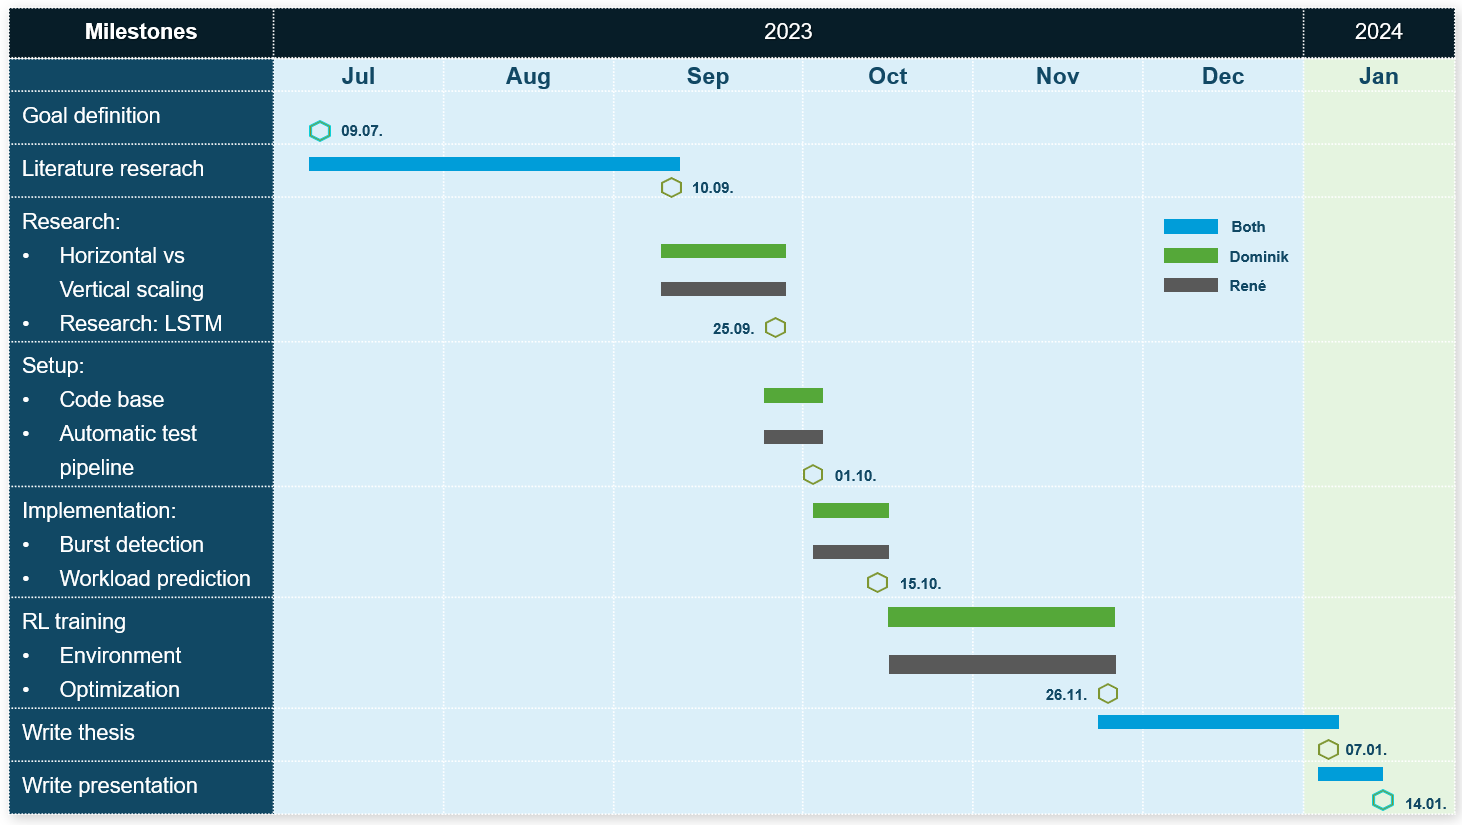
\includegraphics[width=14.5cm,height=7.4cm]{_images/milestones.png}
	\end{figure}
\end{frame}


\subsection{References}
\begin{frame}[allowframebreaks]
	\frametitle{References}
	
	\nocite{bib_uibk_latex}
	
	\bibliographystyle{unsrt}
	\bibliography{main.bib}
\end{frame}


\end{document}